\documentclass[conference]{IEEEtran}
\IEEEoverridecommandlockouts

\usepackage{cite}
\usepackage{amsmath,amssymb}
\usepackage{graphicx}
\usepackage{booktabs}
\usepackage{multirow}
\usepackage{xcolor}
\usepackage{algorithm}
\usepackage{algpseudocode}
\usepackage{tikz}
\usetikzlibrary{arrows.meta,positioning,fit}
\usepackage{url}
\usepackage[hidelinks]{hyperref}

\graphicspath{{figures/}}
\newcommand{\figfile}[2]{\IfFileExists{figures/#2}{\includegraphics[width=#1]{#2}}{\fbox{\parbox{#1}{\centering\vspace{2em}missing: #2\vspace{2em}}}}}

\begin{document}

\title{TrialLens: Evidence-Grounded Clinical Trial Eligibility Screening with a Fine-Tuned Small Language Model and Hand-Built Inference Mechanisms}

\author{\IEEEauthorblockN{Abdullah Rasheed}
\IEEEauthorblockA{Department of Computer Science, FAST National University of Computer and Emerging Sciences\\
Islamabad, Pakistan\\
i230646@isb.nu.edu.pk}}

\maketitle

\begin{abstract}
Deciding whether a patient meets each inclusion and exclusion criterion of a clinical trial is slow manual work, and an assistant is only useful if every decision can be traced to the patient record. We present TrialLens, a criterion-level screening system built on Qwen2.5-1.5B-Instruct and adapted with Low-Rank Adaptation (LoRA) on the TrialGPT Criterion Annotations under a fixed 37/8/8 patient-grouped split. Given a patient note, a criterion type and the criterion text, the model returns one of the expert label categories, including \emph{not enough information} and \emph{not applicable}, together with the IDs of the supporting note sentences. On the held-out test patients, fine-tuning raised accuracy from 0.150 to 0.723, macro-F1 from 0.163 to 0.561 and evidence micro-F1 from 0.207 to 0.496. Around the trained model we implement, from the model's forward pass upward, a key/value (KV) cached decoder, tiled attention with an online softmax, and greedy speculative decoding with a Qwen2.5-0.5B draft. All three reproduce reference outputs, with one documented half-precision near-tie; the KV cache gives up to 6.2$\times$ end-to-end speedup on a T4 GPU, the tiled attention cuts peak attention memory by 26$\times$ at 4k tokens, and speculative decoding, which is slower than greedy decoding on the GPU for reasons we measure and explain, generates long outputs 1.51$\times$ faster on a laptop CPU. A browser application exposes the screening workflow, evidence inspection, report export and live decoding comparisons. The system is an educational prototype, not a clinical enrollment tool.
\end{abstract}

\begin{IEEEkeywords}
clinical trial matching, large language models, LoRA, KV cache, FlashAttention, speculative decoding, evidence attribution
\end{IEEEkeywords}

% ============================================================
\section{Introduction}
Clinical trials specify who may enroll through free-text eligibility criteria. Screening a patient means reading the clinical note against each criterion, and most criteria are either not addressed by the note or need a small clinical inference (a heart rate of 132 satisfies ``at least 90/min''; a 48-year-old man cannot be pregnant). Large language models (LLMs) built on the Transformer~\cite{vaswani2017attention} are a natural fit, and TrialGPT~\cite{jin2024trialgpt} showed that GPT-4 can produce criterion-level judgments with cited evidence that experts largely agree with. A proprietary model is, however, not an option when notes cannot leave the institution or when the system has to run on modest hardware.

This work asks whether a small open-weight decoder, fine-tuned on the expert annotations released with TrialGPT, can make the same kind of criterion-level judgments with sentence-level evidence, and how its inference can be made efficient and verifiable. The problem has four parts:
\begin{enumerate}
\item \textbf{Criterion classification.} Given a patient note $N=\{s_0,\dots,s_m\}$ of numbered sentences, a criterion type $t\in\{\text{inclusion},\text{exclusion}\}$ and criterion text $c$, predict the expert label $y\in\mathcal{Y}_t$, where $\mathcal{Y}_{\text{incl}}=\{$included, not included, not enough information, not applicable$\}$ and $\mathcal{Y}_{\text{excl}}=\{$excluded, not excluded, not enough information, not applicable$\}$.
\item \textbf{Evidence localisation.} Return the set $E\subseteq\{0,\dots,m\}$ of sentence IDs that support $y$, possibly empty.
\item \textbf{Efficient inference.} Implement and validate KV-cached decoding, tiled attention with online softmax, and greedy speculative decoding on freely available hardware.
\item \textbf{Usability.} Deliver a browser application in which a user screens an unseen note against a trial and exports a traceable report.
\end{enumerate}

Our contributions are: (i) a reproducible fine-tuning and evaluation pipeline under the prescribed split with leakage tests, reporting before/after results on identical test cases; (ii) a hand-written Qwen2 forward pass with an explicit, preallocated KV cache that is exactly equivalent to the library model; (iii) a blocked online-softmax attention and a speculative decoder that plug into that forward pass, each tested for token equivalence; (iv) an error analysis that ties recurring mistakes to measurable annotation conventions; and (v) an application with rule-based aggregation and provenance-stamped reports.

% ============================================================
\section{Related Work}
\textbf{Patient--trial matching.} Koopman and Zuccon~\cite{koopman2016test} released the SIGIR 2016 collection of patient descriptions and trials that underlies the patients used here. TrialGPT~\cite{jin2024trialgpt} decomposes matching into criterion-level prediction with GPT-4, then ranks trials; its expert annotation of 1{,}015 criterion predictions is our benchmark. Wornow et al.~\cite{wornow2024zeroshot} show zero-shot GPT-4 matching on the n2c2 cohort and stress cost and context limits. Both rely on proprietary models; our setting replaces them with a 1.5B-parameter open model and supervised adaptation, and we never feed the stored GPT-4 outputs to our model.

\textbf{Small decoders and adaptation.} Qwen2.5~\cite{qwen2025qwen25} and Llama~3~\cite{dubey2024llama3} provide open decoders from 0.5B parameters upward, with grouped-query attention (GQA)~\cite{ainslie2023gqa}, rotary position embeddings (RoPE)~\cite{su2024roformer}, RMSNorm~\cite{zhang2019rmsnorm} and SwiGLU feed-forward layers~\cite{shazeer2020glu}. LoRA~\cite{hu2022lora} trains low-rank updates to frozen weights; QLoRA~\cite{dettmers2023qlora} additionally quantises the base model to 4 bits. With a 1.5B model the fp16 base fits a 16\,GB GPU, so we use plain LoRA and avoid the extra quantisation error and the bitsandbytes dependency.

\textbf{Efficient inference.} Autoregressive decoding is dominated by re-reading weights and past keys/values; caching keys/values turns each step into a single-token pass whose memory grows linearly with context~\cite{pope2023efficiently}, and PagedAttention~\cite{kwon2023pagedattention} manages that memory in blocks for serving. The online softmax~\cite{milakov2018online} computes a softmax in one pass with a running maximum and normaliser; Rabe and Staats~\cite{rabe2021selfattention} use it to make attention memory sub-quadratic, and FlashAttention~\cite{dao2022flashattention,dao2024flashattention2} fuses it into tiled GPU kernels that avoid materialising the score matrix. Speculative decoding~\cite{leviathan2023fast,chen2023accelerating} lets a cheap draft model propose tokens that the target verifies in one pass; with greedy acceptance the output is identical to the target's greedy output, and the speedup depends on the acceptance rate and on the draft-to-target cost ratio. We implement simplified versions of all three to validate them and to measure where they help.

% ============================================================
\section{Materials and Methods}

\subsection{Dataset and split}
The TrialGPT Criterion Annotations contain 1{,}015 criterion-level records for 53 patients from the SIGIR collection~\cite{koopman2016test} and 103 trials. Each record has the numbered patient note, criterion type and text, the expert eligibility label and expert evidence sentence IDs, plus GPT-4's prediction, explanation and an explanation-correctness grade. We keep only the note, criterion type, criterion text, expert label and expert evidence through an explicit column allow-list; a unit test asserts that no \texttt{gpt4\_*} field reaches a processed record. The dataset's own \texttt{training} flag is also ignored.

Unique patient IDs are sorted, shuffled with \texttt{numpy.random.default\_rng(42)}, and the first 37, next 8 and last 8 patients form train, validation and test. Tests check the 37/8/8 sizes, that no patient appears in two splits, that every annotation is used exactly once, and that \texttt{rng.permutation} reproduces the same order. One record (annotation 883) has an empty criterion text and is dropped and logged in the published manifest. Table~\ref{tab:data} summarises the result. The label distribution is highly skewed: \emph{excluded} has 10 examples in the whole dataset and none in the test split, and 60\% of all records have no expert evidence.

\begin{table}[t]
\centering
\caption{Patient-grouped split (seed 42). NEI = not enough information.}
\label{tab:data}
\begin{tabular}{lrrr}
\toprule
 & Train & Val & Test \\
\midrule
Patients & 37 & 8 & 8 \\
Criterion records & 602 & 206 & 206 \\
\quad inclusion / exclusion & 215 / 387 & 66 / 140 & 75 / 131 \\
Records without gold evidence & 348 & 116 & 145 \\
\midrule
included & 88 & 35 & 27 \\
not included & 13 & 3 & 7 \\
excluded & 8 & 2 & 0 \\
not excluded & 291 & 101 & 91 \\
NEI & 174 & 53 & 66 \\
not applicable & 28 & 12 & 15 \\
\bottomrule
\end{tabular}
\end{table}

\subsection{Model selection}
Table~\ref{tab:models} compares the candidates we considered for a free 16\,GB T4 for training and a 16\,GB-RAM laptop CPU for the application. Qwen2.5-1.5B-Instruct was selected: it is Apache-2.0 licensed and ungated, it has the smallest KV cache per token of the candidates thanks to two KV heads, its fp32 weights (6.2\,GB) leave room for a draft model in 16\,GB of RAM, and the 0.5B sibling shares the same tokenizer and vocabulary, which speculative decoding requires. Qwen2.5-3B was rejected because its fp32 weights alone (12.4\,GB) would make CPU inference impractical and its licence is research-only; Llama-3.2 was rejected because of its gated licence and an 8-KV-head cache that is larger per token. The model uses a 32{,}768-token context; our longest training example is 634 tokens.

\begin{table}[t]
\centering
\caption{Open-weight decoder candidates. KV is fp16 cache size per token; weights are fp16.}
\label{tab:models}
\setlength{\tabcolsep}{3pt}
\begin{tabular}{lrrrrrl}
\toprule
Model & Params & Layers & Q/KV & KV/tok & Weights & Licence \\
\midrule
Qwen2.5-0.5B & 0.49B & 24 & 14/2 & 12\,KB & 1.0\,GB & Apache-2.0 \\
\textbf{Qwen2.5-1.5B} & \textbf{1.54B} & 28 & 12/2 & 28\,KB & 3.1\,GB & Apache-2.0 \\
Qwen2.5-3B & 3.09B & 36 & 16/2 & 36\,KB & 6.2\,GB & Research \\
Llama-3.2-1B & 1.24B & 16 & 32/8 & 32\,KB & 2.5\,GB & Llama 3.2 \\
Llama-3.2-3B & 3.21B & 28 & 24/8 & 112\,KB & 6.4\,GB & Llama 3.2 \\
\bottomrule
\end{tabular}
\end{table}

\subsection{Input and output format}
The prompt is the model's chat template with a system message stating the task rules (use only facts in the note; missing facts are never proof either way; \emph{not applicable} when the criterion cannot apply), followed by the numbered note, the criterion type, the criterion text and the four allowed labels for that type. The patient note precedes the criterion so that all criteria for one patient share a prompt prefix (Section~\ref{sec:app}). The target is a single JSON object, evidence first:
\begin{center}\small\texttt{\{"evidence\_ids": [0, 2], "label": "included"\}}\end{center}
Placing evidence before the label conditions the label on the cited sentences. The dataset contains no expert explanations (only GPT-4's), so the model is not trained to write explanations; the application composes each explanation deterministically from the predicted label and the cited sentences. Prompts average 324 tokens (maximum 607) and targets 16 tokens; at a 1{,}024-token limit no example is truncated, so no evidence is ever cut from the note. Model output is parsed by taking the first balanced JSON object; an unparseable output or a label outside the criterion type's set is scored as \emph{invalid} and counted wrong, and cited IDs that do not exist in the note are dropped and logged.

\subsection{Fine-tuning}
We train LoRA adapters on all seven projection matrices of every layer (Table~\ref{tab:hparams}). The objective is next-token cross-entropy on the answer tokens only: prompt positions get label $-100$, so the model is not trained to reproduce notes. The base weights are kept in fp32 with fp16 autocast and loss scaling, which fits in 12.0\,GB on a T4 with gradient checkpointing. After every epoch the adapter decodes the full validation split greedily and the epoch with the best validation macro-F1 is kept; this rule was fixed before training and the test split is never read by the training script.

To address the label imbalance we compare three runs: rank 16 (\texttt{r16}), rank 8 (\texttt{r8}), and rank 16 with oversampling (\texttt{os40}), which repeats records of any label with fewer than 40 training examples until it has 40 per epoch (adding 71 records).

\begin{table}[t]
\centering
\caption{Fine-tuning configuration (shared by all runs unless noted).}
\label{tab:hparams}
\begin{tabular}{ll}
\toprule
Adapter & LoRA $r{=}16$, $\alpha{=}32$, dropout 0.05 \\
Target modules & q, k, v, o, gate, up, down projections \\
Trainable parameters & 18.5M (1.2\% of 1.54B) \\
Optimiser & AdamW, lr $2\times10^{-4}$, no weight decay \\
Schedule & cosine, 5\% warm-up, 4 epochs \\
Batch & 4 $\times$ 4 accumulation = 16 \\
Precision & fp32 master weights, fp16 autocast \\
Max length / truncation & 1{,}024 tokens / none needed \\
Hardware & 1$\times$ Tesla T4 16\,GB (Kaggle), seed 42 \\
\bottomrule
\end{tabular}
\end{table}

\subsection{System architecture}
Fig.~\ref{fig:arch} shows how the components fit together. The Hugging Face model is used only as a container for weights: every forward pass in evaluation benchmarks and in the application runs through our own decoder.

\begin{figure}[t]
\centering
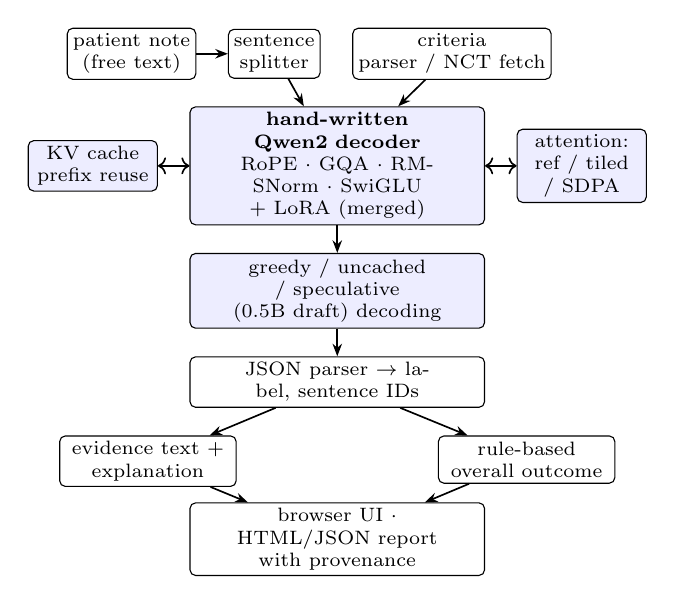
\begin{tikzpicture}[font=\scriptsize, node distance=3.5mm and 4mm,
  box/.style={draw, rounded corners=2pt, align=center, minimum height=6mm, inner sep=2pt, fill=white},
  hi/.style={box, fill=blue!7}, arr/.style={-{Stealth[length=1.6mm]}, semithick}]
\node[box] (note) {patient note\\(free text)};
\node[box, right=of note] (split) {sentence\\splitter};
\node[box, right=of split] (crit) {criteria\\parser / NCT fetch};
\node[hi, below=of split, xshift=8mm, text width=36mm] (dec) {\textbf{hand-written Qwen2 decoder}\\RoPE $\cdot$ GQA $\cdot$ RMSNorm $\cdot$ SwiGLU\\+ LoRA (merged)};
\node[hi, left=of dec, text width=15mm] (kv) {KV cache\\prefix reuse};
\node[hi, right=of dec, text width=15mm] (att) {attention:\\ref / tiled / SDPA};
\node[hi, below=of dec, text width=36mm] (spec) {greedy / uncached / speculative\\(0.5B draft) decoding};
\node[box, below=of spec, text width=36mm] (parse) {JSON parser $\to$ label, sentence IDs};
\node[box, below left=3.5mm and -6mm of parse, text width=21mm] (expl) {evidence text +\\explanation};
\node[box, below right=3.5mm and -6mm of parse, text width=21mm] (agg) {rule-based\\overall outcome};
\node[box, below=12mm of parse, text width=36mm] (rep) {browser UI $\cdot$ HTML/JSON report\\with provenance};
\draw[arr] (note) -- (split); \draw[arr] (split) -- (dec); \draw[arr] (crit) -- (dec);
\draw[arr, <->] (kv) -- (dec); \draw[arr, <->] (att) -- (dec);
\draw[arr] (dec) -- (spec); \draw[arr] (spec) -- (parse);
\draw[arr] (parse) -- (expl); \draw[arr] (parse) -- (agg);
\draw[arr] (expl) -- (rep); \draw[arr] (agg) -- (rep);
\end{tikzpicture}
\caption{TrialLens pipeline. Shaded blocks are implemented from the model's weights upward.}
\label{fig:arch}
\end{figure}

\subsection{KV-cached decoding}
Our decoder applies, per layer, RMSNorm, the $q,k,v$ projections, RoPE, attention over grouped heads, the output projection, RMSNorm and the SwiGLU MLP, then the final norm and the tied LM head. The cache is a preallocated tensor pair of shape $[L, B, H_{kv}, T_{\max}, d]$ with a length pointer $\ell$. Algorithm~\ref{alg:kv} gives the loop.

\emph{Positions.} A token's rotary angle depends only on its absolute position. Prefill rotates prompt tokens at positions $0..P{-}1$; a decode step rotates its single query and key at position $\ell$, exactly as a full recomputation would, so cached keys are never re-rotated.

\emph{Masking.} The attention functions receive a query offset $o=\ell$: query $i$ at absolute position $o+i$ may attend keys $0..o+i$. Prefill uses a $P\times P$ causal mask; a single decode step attends to every cached key; a multi-token chunk on top of a cache (speculative verification, shared-prefix reuse) gets the causal mask shifted by $o$. Passing \texttt{is\_causal=True} to a fused kernel would be wrong in that last case, because it assumes queries start at key 0; our SDPA wrapper builds the offset mask explicitly.

\emph{Growth.} Writing a step is a slice assignment at $[\ell, \ell{+}T)$, so there is no per-token concatenation, and rolling back is just $\ell\leftarrow\ell'$. Memory grows as $2LH_{kv}d\cdot b$ bytes per token: 28\,KB in fp16 and 56\,KB in fp32 for Qwen2.5-1.5B.

\emph{Reference path.} The uncached decoder re-runs the full forward pass on the whole sequence for every new token, with the same functions and no cache.

\begin{algorithm}[t]
\caption{Greedy decoding with an explicit KV cache}
\label{alg:kv}
\begin{algorithmic}[1]
\Require prompt $x_{0..P-1}$, cache $C$ (length $\ell$), steps $n$
\State $C.\ell \gets 0$;\quad $z \gets \Call{Forward}{x_{0..P-1}, C, \text{start}{=}0}$ \Comment{writes $P$ entries}
\State $y_1 \gets \arg\max z_{P-1}$
\For{$t = 2$ \textbf{to} $n$}
  \State $z \gets \Call{Forward}{y_{t-1}, C, \text{start}{=}C.\ell}$ \Comment{1 query, RoPE at pos.\ $C.\ell$}
  \State $y_t \gets \arg\max z_0$ \Comment{$C.\ell$ grows by 1}
  \If{$y_t = \text{EOS}$} \textbf{break} \EndIf
\EndFor
\State \Return $y$
\end{algorithmic}
\end{algorithm}

\subsection{Tiled attention with online softmax}
The reference attention computes $S=QK^\top/\sqrt{d}$, masks future keys with $-\infty$, subtracts the row maximum, exponentiates and normalises, all in fp32. The tiled variant (Algorithm~\ref{alg:tiled}) processes queries in blocks of $B_q$ and keys in blocks of $B_k$, keeping for each query row a running maximum $m$, a running normaliser $l$ and an unnormalised accumulator $A$. When a new tile raises the maximum, the old $l$ and $A$ are rescaled by $e^{m-m'}$. Key blocks that lie entirely in the causal future of a query block are skipped. A row that is fully masked within one tile would produce $e^{-\infty-(-\infty)}$; we shift by 0 instead of $-\infty$ in that case to avoid NaNs. Only a $B_q\times B_k$ tile of scores exists at a time, so score memory falls from $O(T_qT_k)$ to $O(B_qB_k)$ per head.

\begin{algorithm}[t]
\caption{Tiled causal attention with online softmax (one head)}
\label{alg:tiled}
\begin{algorithmic}[1]
\For{each query block $Q_b$ (rows $r$)}
  \State $m \gets -\infty$, $l \gets 0$, $A \gets 0$
  \For{each key block $K_c, V_c$ not fully in the future of $Q_b$}
    \State $S \gets Q_bK_c^\top/\sqrt{d}$; mask keys after $o+r$ with $-\infty$
    \State $m' \gets \max(m, \text{rowmax}(S))$
    \State $P \gets \exp(S - m')$;\quad $\gamma \gets \exp(m - m')$
    \State $l \gets \gamma l + \text{rowsum}(P)$;\quad $A \gets \gamma A + PV_c$;\quad $m \gets m'$
  \EndFor
  \State $O_b \gets A / l$
\EndFor
\end{algorithmic}
\end{algorithm}

\subsection{Greedy speculative decoding}
The draft (Qwen2.5-0.5B-Instruct) and target share the same 151{,}936-entry vocabulary, which the benchmark asserts before running. Each round (Algorithm~\ref{alg:spec}) drafts $k$ tokens, verifies them with one target pass over $k{+}1$ positions, accepts the longest agreeing prefix and appends the target's own token at the first disagreement, or a bonus token when all $k$ agree. Every committed token is therefore the target's greedy choice. Both caches contain entries for rejected tokens after a round; they are cropped to the accepted length, and each model keeps a short list of committed tokens it has not yet processed (one for the target; one or two for the draft, which never ran a pass on its own last proposal). We also fine-tune the draft on the same training split with the same recipe (8.8M LoRA parameters) to raise acceptance on the task.

\begin{algorithm}[t]
\caption{Greedy speculative decoding with cache synchronisation}
\label{alg:spec}
\begin{algorithmic}[1]
\State prefill target and draft on the prompt; $y \gets [\arg\max]$; pending$_T$, pending$_D \gets [y_1]$
\While{$|y| < n$ and last token $\neq$ EOS}
  \State $\ell_T, \ell_D \gets$ cache lengths
  \State draft $d_1..d_k$ greedily (first pass also feeds pending$_D$)
  \State $g_0..g_k \gets \arg\max$ of one target pass on pending$_T\Vert d_{1..k}$
  \State $a \gets$ largest $j$ with $d_i = g_{i-1}$ for all $i\le j$
  \State append $d_{1..a}$ and $g_a$ to $y$
  \State crop target cache to $\ell_T + 1 + a$; draft cache to $\ell_D + |\text{pending}_D| + \min(a, k{-}1)$
  \State pending$_T \gets [g_a]$;\quad pending$_D \gets [d_k, g_a]$ if $a{=}k$ else $[g_a]$
\EndWhile
\end{algorithmic}
\end{algorithm}

\subsection{Application workflow}\label{sec:app}
The Gradio application (started with \texttt{start.bat}, which builds the environment on first run) accepts a free-text or numbered note and criteria typed in the ClinicalTrials.gov layout or fetched by NCT number from the public ClinicalTrials.gov API. Free text is split into sentences that are numbered for citation. Inputs are validated (empty note, missing section headers, over-long notes, malformed trial IDs) with messages instead of crashes. The system prompt and note are prefilled once and their KV cache is reused for every criterion; we verified on all 808 train and validation prompts that tokenising prefix and suffix separately yields exactly the same tokens as tokenising the whole prompt, so this reuse cannot change predictions. Each criterion is shown as a card with its label, the cited sentences, an explanation, and a flag when a definite decision has no cited evidence. The preliminary patient-level outcome is an aggregation by fixed rules, not a labelled ground truth: any \emph{not included} or \emph{excluded} gives \emph{Likely ineligible}; otherwise any \emph{not enough information} or unreadable answer gives \emph{Needs review}; otherwise \emph{Potentially eligible}. Reports download as HTML or JSON with the model, adapter hash, decoding settings, git commit and a hash of the note. An inference lab runs the decoding modes and attention implementations live on the user's machine and checks token equality. Fig.~\ref{fig:app} shows the screening view on a validation patient and Fig.~\ref{fig:lab} a live decoding comparison. A recorded demonstration of the full workflow is available at \href{https://youtu.be/StV4EAdW9mc}{\texttt{youtu.be/StV4EAdW9mc}}.

\begin{figure*}[t]
\centering
\figfile{0.86\textwidth}{app_screening_crop.png}
\caption{Screening view on a validation patient (laptop CPU). Left: note, criteria and settings. Right: the rule-based preliminary outcome, report downloads and criterion cards with the label, cited sentences, an explanation built from them, and the expert annotation shown only for validation examples. The model agrees with the experts on 3 of the 6 criteria here; the disagreements are \emph{not included} and \emph{not applicable} cases discussed in Section~\ref{sec:errors}.}
\label{fig:app}
\end{figure*}

\begin{figure*}[t]
\centering
\figfile{0.9\textwidth}{app_lab_crop.png}
\caption{Inference lab on the laptop CPU after a warm-up run (294-token prompt, 16 generated tokens, fp32): live timings of each decoding mode, all producing tokens identical to KV-cached greedy decoding.}
\label{fig:lab}
\end{figure*}

% ============================================================
\section{Experimental Setup and Metrics}
\textbf{Classification.} Accuracy, per-class precision, recall and F1, macro-F1 and confusion matrices, overall and separately for inclusion and exclusion criteria. Macro-F1 averages over the labels that occur in the gold labels of the scope; a label with no gold examples (\emph{excluded} on test) has undefined recall and is reported but not averaged. Invalid outputs are always wrong.

\textbf{Evidence.} Micro precision, recall and F1 sum true positives, false positives and false negatives over all records, so records with empty gold evidence contribute only false positives. Macro scores average per-record precision, recall and F1 over records whose gold set is non-empty; an empty prediction there scores 0. Records with empty gold evidence are scored separately as \emph{abstention accuracy}: the share where the model also cited nothing.

\textbf{Decoding.} All accuracy results use deterministic greedy decoding (no sampling, one beam, at most 64 new tokens) through the same prompt, so the before/after comparison changes only the weights. Benchmarks report the median of three synchronised runs after one warm-up, with peak memory from \texttt{torch.cuda.max\_memory\_allocated} on GPU (after resetting the peak, excluding weights) and sampled process RSS on CPU. GPU numbers come from one Tesla T4 (fp16); CPU numbers from an Intel i5-1145G7 laptop (4 cores, fp32).

% ============================================================
\section{Results and Discussion}

\subsection{Fine-tuning and model selection}
Fig.~\ref{fig:curves} shows training loss falling smoothly for all three runs while validation loss reaches its minimum at epoch 2 and then rises, a sign of over-fitting the answer format on 602 examples. Validation macro-F1 does not track validation loss: it is driven by a handful of rare-label examples. Table~\ref{tab:val} lists the selected epoch of each run. Oversampling (\texttt{os40}) gave the best macro-F1 (0.564) at epoch 2, and halving the rank (\texttt{r8}) came within 0.011 with half the trainable parameters. We kept \texttt{os40} under the pre-registered rule, but the margin is about one example: validation holds only two \emph{excluded} and three \emph{not included} records, so one correct prediction moves macro-F1 by roughly 0.1. The fine-tuned 0.5B draft reached 0.447, close to the 1.5B rank-16 run.

\begin{figure*}[t]
\centering
\figfile{\textwidth}{training_curves.pdf}
\caption{Training loss, validation loss and validation macro-F1 per epoch for the three LoRA runs. Stars mark the epoch kept by the selection rule.}
\label{fig:curves}
\end{figure*}

\begin{table}[t]
\centering
\caption{Validation results (206 criteria) at the selected epoch.}
\label{tab:val}
\setlength{\tabcolsep}{4pt}
\begin{tabular}{lrrrrr}
\toprule
Run & Trainable & Epoch & Acc. & Macro-F1 & Ev.\ F1 \\
\midrule
Base 1.5B (zero-shot) & -- & -- & 0.121 & 0.121 & 0.142 \\
r16 & 18.5M & 4 & 0.748 & 0.444 & 0.515 \\
\textbf{os40} & 18.5M & 2 & \textbf{0.762} & \textbf{0.564} & 0.459 \\
r8 & 9.2M & 3 & 0.752 & 0.553 & 0.498 \\
Draft 0.5B, r16 & 8.8M & 3 & 0.738 & 0.447 & 0.449 \\
\bottomrule
\end{tabular}
\end{table}

\subsection{Held-out test results}
The test split was evaluated once, for the zero-shot base model and the selected adapter, with identical prompts and decoding (Table~\ref{tab:test}). The base model almost always answered \emph{not applicable} (182 of 206 predictions), which explains its 0.150 accuracy; the instruction-tuned model understands the JSON format (no invalid outputs) but not the label scheme. Fine-tuning raised accuracy to 0.723 and macro-F1 to 0.561, with inclusion criteria at 0.787 accuracy and exclusion criteria at 0.687.

\begin{table}[t]
\centering
\caption{Held-out test results (206 criteria, 8 patients), greedy decoding. Ev.\ = evidence; Abst.\ = abstention accuracy on 145 records without gold evidence.}
\label{tab:test}
\setlength{\tabcolsep}{3.2pt}
\begin{tabular}{llrrrrrr}
\toprule
 & Scope & Acc. & M-F1 & Ev.\ P & Ev.\ R & Ev.\ F1 & Ev.\ mF1 \\
\midrule
\multirow{3}{*}{Base} & all & 0.150 & 0.163 & 0.211 & 0.202 & 0.207 & 0.097 \\
 & incl. & 0.227 & 0.181 & 0.221 & 0.306 & 0.257 & 0.131 \\
 & excl. & 0.107 & 0.072 & 0.000 & 0.000 & 0.000 & 0.000 \\
\midrule
\multirow{3}{*}{os40} & all & \textbf{0.723} & \textbf{0.561} & 0.846 & 0.351 & 0.496 & 0.408 \\
 & incl. & 0.787 & 0.424 & 0.838 & 0.500 & 0.626 & 0.508 \\
 & excl. & 0.687 & 0.517 & 1.000 & 0.062 & 0.118 & 0.125 \\
\midrule
\multicolumn{8}{l}{Abstention accuracy: base 0.979, os40 1.000.} \\
\bottomrule
\end{tabular}
\end{table}

Per-class F1 (Fig.~\ref{fig:beforeafter}) shows the gains are broad: \emph{not excluded} from 0.04 to 0.80, \emph{not enough information} from 0 to 0.62 and \emph{not applicable} from 0.15 to 0.52. \emph{Not included} stays at zero: all seven test cases were predicted as \emph{not enough information} (Fig.~\ref{fig:confusion}). Evidence citation is precise (0.846) but conservative (recall 0.351): the model never cites a sentence when the experts cited none (abstention 1.000), but it also omits evidence for many exclusion decisions, where experts cited sentences only 16 times out of 131.

\begin{figure}[t]
\centering
\figfile{\columnwidth}{before_after_f1.pdf}
\caption{Per-class test F1 of the same model before and after fine-tuning. \emph{excluded} has no test examples and is omitted.}
\label{fig:beforeafter}
\end{figure}

\begin{figure}[t]
\centering
\figfile{0.78\columnwidth}{confusion_test.pdf}
\caption{Test confusion matrix of the fine-tuned model (rows: expert label). No test record is labelled or predicted \emph{excluded}, and no output was invalid.}
\label{fig:confusion}
\end{figure}

\subsection{Error analysis}\label{sec:errors}
Of 206 test predictions, 57 have the wrong label and 22 more have the right label but miss all of the experts' evidence. Table~\ref{tab:errors} lists representative cases; the full set is produced by \texttt{scripts/error\_analysis.py}.

\begin{table*}[t]
\centering
\caption{Representative test errors of the fine-tuned model. G = expert label and evidence, P = prediction.}
\label{tab:errors}
\small
\begin{tabular}{p{0.3cm}p{2.6cm}p{4.5cm}p{3.1cm}p{5.4cm}}
\toprule
\# & Category & Criterion (abridged) & G $\to$ P & Analysis \\
\midrule
1 & Missing info read as negative (24) & Excl.: severe renal impairment (GFR $<$50\%) & NEI [] $\to$ not excluded [] & The note never mentions renal function. The model followed the dataset majority (below) instead of abstaining. \\
2 & Missing info read as negative & Excl.: patients were moribund & NEI [0--4] $\to$ not excluded [] & Experts cited the whole presentation as relevant yet undecidable; the model judged ``not moribund'' without citing anything. \\
3 & Missed negative (7) & Incl.: undergoing elective carotid endarterectomy & not included [] $\to$ NEI [] & The note describes a cardiac catheterisation. Experts inferred that the listed surgery is not happening; the model would not infer a negative from context. All 7 \emph{not included} test cases fail this way. \\
4 & Over-abstention (16) & Incl.: heart rate of at least 90/min & included [2] $\to$ NEI [3] & Sentence 2 says ``tachycardic'', which implies $\geq$90/min; the model needs the explicit number and cites the blood-pressure sentence instead. \\
5 & Over-abstention & Incl.: diagnosed with shock or ARDS & included [2,3] $\to$ NEI [] & BP 80/60 with tachycardia and tachypnoea indicates shock; the clinical inference is missed. \\
6 & Over-abstention & Excl.: less than 18 years of age & not excluded [0] $\to$ NEI [] & Sentence 0 states the patient is 40. A plain extraction failure on a simple criterion. \\
7 & Contradictory annotation & Excl.: pregnant women or women of childbearing age without contraception & not excluded [0] $\to$ N/A [] & The patient is a 48-year-old man. In train/val, 17 of 18 pregnancy criteria for male patients are labelled N/A; this test label is the outlier, and the model follows the majority. \\
8 & Missing info read as positive (1) & Incl.: sore throat or odynophagia with $\geq$2 clinical signs & NEI [0] $\to$ included [0,1,2] & A child with dysphagia, drooling and fever. The model cites plausible signs; the experts judged the evidence insufficient. A borderline, arguably defensible error. \\
9 & Unsupported correct (22) & Excl.: inability to answer questions & not excluded [5] $\to$ not excluded [] & Right label, but the experts' evidence (consent and compliance sentence) is not cited, so the decision is not traceable. The app flags such cards. \\
10 & Applicability (9) & Excl.: previous tonsillectomy & N/A [] $\to$ not excluded [] & N/A versus \emph{not excluded} is decided inconsistently by annotators when a criterion is unrelated to the patient. \\
\bottomrule
\end{tabular}
\end{table*}

Two measurable annotation conventions explain many of these errors. First, among the 381 train and validation exclusion criteria without gold evidence, experts wrote \emph{not excluded} 286 times (75\%), \emph{not enough information} 68 times and \emph{not applicable} 27 times. In other words, the reference labels themselves usually treat an unmentioned exclusion condition as absent. The model learned this majority, which yields 24 test errors where the experts chose \emph{not enough information} instead, and an inclusion/exclusion asymmetry: \emph{not enough information} recall is 0.974 for inclusion criteria but 0.107 for exclusion criteria. Because absent evidence should never be taken as proof of eligibility or ineligibility, the application marks every definite decision that has no cited sentence as unsupported and routes the patient to \emph{Needs review} when any criterion is undecided. Second, pregnancy-type criteria for male patients are \emph{not applicable} in 17 of 18 cases, so error 7 reflects label noise rather than model failure. The remaining errors (3--6) are genuine reasoning gaps: the 1.5B model does not infer negatives from context or translate clinical descriptions (``tachycardic'') into numeric thresholds.

\subsection{KV-cached decoding}\label{sec:kvres}
On the real 1.5B model our forward pass with the SDPA backend reproduces the library's logits exactly (maximum difference 0 on a 200-token input), and the reference and tiled backends stay within $4.4\times10^{-5}$ with identical arg-max at every position. Unit tests on a small random Qwen2 model check cached against uncached greedy tokens at three prompt/output lengths for all three attention backends, cached logits against full recomputation, cache cropping, and agreement with \texttt{generate}. On the laptop CPU in fp32, cached and uncached decoding produced identical tokens in all four configurations, with 2.6$\times$ to 8.1$\times$ end-to-end speedups.

Table~\ref{tab:kv} and Fig.~\ref{fig:kv} give the T4 results in fp16. Cached decoding holds about 28 tokens/s regardless of prompt length because each step processes one token, while the uncached path falls from 27.9 to 4.4 tokens/s as it reprocesses ever longer sequences. At a 128-token prompt the two are almost equally fast: our hand-written decoder launches several hundred small kernels per step, so a single-token pass and a 160-token pass both cost about one launch-bound step. The benefit appears once the prompt is long enough to make recomputation compute-bound, reaching 6.2$\times$ at 1{,}024 tokens. The cache costs 28\,KB per token, 31.5\,MB at 1{,}152 positions, which shows up as a slightly higher peak memory than the uncached path.

\begin{table}[t]
\centering
\caption{KV-cached vs uncached greedy decoding, Qwen2.5-1.5B + LoRA, T4 fp16, median of 3.}
\label{tab:kv}
\setlength{\tabcolsep}{3pt}
\begin{tabular}{rrrrrrrc}
\toprule
In & Out & \multicolumn{2}{c}{Prefill ms} & \multicolumn{2}{c}{Decode tok/s} & Speedup & Tokens \\
 & & cache & none & cache & none & & equal \\
\midrule
128 & 32 & 32.8 & 30.8 & 28.6 & 27.9 & 1.02 & yes \\
128 & 128 & 31.8 & 33.2 & 28.8 & 22.7 & 1.26 & 54/128$^\ast$ \\
512 & 32 & 76.9 & 101.9 & 28.4 & 8.1 & 3.35 & yes \\
512 & 128 & 84.4 & 102.5 & 28.1 & 7.8 & 3.54 & yes \\
1024 & 32 & 183.6 & 202.7 & 28.8 & 4.5 & 5.64 & yes \\
1024 & 128 & 182.9 & 197.9 & 28.4 & 4.4 & 6.16 & yes \\
\bottomrule
\multicolumn{8}{l}{\footnotesize $^\ast$identical for the first 54 tokens; see text.}
\end{tabular}
\end{table}

\begin{figure*}[t]
\centering
\figfile{\textwidth}{kv_cache.pdf}
\caption{Decode throughput with and without the KV cache on a T4. Labels give the end-to-end speedup; $\ast$ marks the run with a token mismatch.}
\label{fig:kv}
\end{figure*}

\emph{Investigating the mismatch.} In the 128/128 run the two paths agree for 54 tokens and then diverge. The benchmark logs the gap between the best and second-best logit at the first differing step: 0.0156, which is exactly $2^{-6}$, the spacing between adjacent fp16 numbers in $[16, 32)$, the range of the top logits. The two candidates were one fp16 rounding step apart. The cached path computes each step with a 1-row matrix product while the uncached path computes the same row inside a 160-row product; the different reduction order changes the last bit, which flips this near-tie, after which the sequences legitimately diverge. The same 128/128 configuration in fp32 on CPU produces identical tokens at all 128 steps (8.2$\times$ faster with the cache), even though its closest near-tie was tighter (a gap of 0.0085), because fp32 resolves differences far below that; every other fp16 configuration also matched exactly. We therefore attribute the mismatch to half-precision arithmetic rather than to the cache logic.

\subsection{Tiled attention}
On random inputs with Qwen's 12 heads of dimension 128, the reference, tiled (block sizes 32, 64, 128) and SDPA outputs agree with a float64 computation to at most $1.7\times10^{-6}$ in fp32 on CPU, across full causal prompts, a single decode query on a 300-key cache and a 5-query verification chunk with a 128-token offset. In fp16 on the T4 all methods share the same worst error, $9.6\times10^{-4}$ (SDPA $1.1\times10^{-3}$), which is the precision of fp16 outputs rather than of the algorithm. Unit tests also cover ragged final blocks, block sizes that do not divide the sequence (7$\times$13), scores of magnitude $10^4$ that would overflow a naive exponential, and fp16 inputs.

Fig.~\ref{fig:attention} shows the trade-off. Memory behaves as designed: at 4{,}096 tokens the reference materialises 12 score matrices and needs 2{,}320\,MB beyond its inputs, while the tiled version with 128$\times$128 tiles needs 88.5\,MB (26$\times$ less) and grows linearly. Speed does not: the tiled version is 3.4$\times$ slower than the reference at 4k and up to 55$\times$ slower than SDPA, and smaller tiles are slower still (3.7\,s with 32$\times$32 tiles). Each tile is a separate set of PyTorch kernel launches with its intermediate results written to GPU memory, whereas FlashAttention keeps the tile in on-chip SRAM inside one fused kernel; our implementation reproduces the algorithm but not the memory hierarchy that makes it fast, so on the GPU it is a correctness and memory demonstration rather than a speed-up. The CPU tells a different story: with 128-wide tiles the tiled version took 45\,ms at 1{,}024 tokens against 86\,ms for the reference, because each 0.75\,MB tile of scores stays in the processor cache while the reference writes and re-reads a 48\,MB score matrix; with 32-wide tiles the per-tile overhead dominates again (188\,ms). PyTorch's fused CPU kernel remained fastest (17\,ms).

\begin{figure*}[t]
\centering
\figfile{\textwidth}{attention.pdf}
\caption{Causal attention runtime and peak extra memory on a T4 (fp16, 12 heads $\times$ 128). The tiled version trades speed for memory; PyTorch's fused kernel wins on both.}
\label{fig:attention}
\end{figure*}

\subsection{Speculative decoding}
Every speculative run, on 10 criterion prompts and 10 free-text summary prompts for $k\in\{1,2,4,6,8\}$ and with both drafts, produced exactly the target's greedy tokens (200/200). Fig.~\ref{fig:spec} shows the trade-off on the criterion task. The stock draft accepts 60--83\% of proposals; the fine-tuned draft accepts 97--100\%, committing up to 4.9 tokens per target pass. Yet on the T4 neither is faster than greedy decoding (0.59--1.04$\times$).

The reason is the draft-to-target cost ratio $c$. With acceptance rate $\alpha$ and $k$ drafts, the expected speedup is $\frac{1-\alpha^{k+1}}{(1-\alpha)(ck+1)}$~\cite{leviathan2023fast}. On the GPU our decoder is limited by kernel launches per layer rather than by arithmetic (Section~\ref{sec:kvres}), so a decode step costs roughly in proportion to the number of layers, and the 24-layer draft is estimated to cost $c\approx24/28\approx0.86$ of a 28-layer target step. Even at $\alpha=1$ and $k=4$ that bounds the speedup at $5/4.4\approx1.1$, and the larger verification pass and cache bookkeeping absorb the rest. Free-text summaries, where acceptance falls to 69--94\%, behave the same way.

The CPU behaves differently (Table~\ref{tab:spec}). A CPU decode step is limited by reading the weights from memory, so $c$ approaches the parameter ratio, about 0.33. There, speculative decoding with the fine-tuned draft generated 48-token summaries 1.51$\times$ faster than greedy decoding at $k=2$ (88\% acceptance), with identical tokens. On the criterion task it was still slower (0.69--0.94$\times$) despite 100\% acceptance: answers are only about 15 tokens long, so the extra draft prefill over a 340-token prompt costs more than drafting saves. Larger $k$ also hurt on the CPU, because verifying more tokens and drafting proposals that are later rejected both add work. Speculative decoding therefore helps for long outputs with a draft that is much cheaper than the target, which is not the regime of this short-answer task.

\begin{table}[t]
\centering
\caption{Speculative decoding vs KV-cached greedy decoding. Speedup is end-to-end; all runs produced the greedy tokens.}
\label{tab:spec}
\setlength{\tabcolsep}{3.5pt}
\begin{tabular}{llrrrr}
\toprule
Setting & Draft & $k$ & Accept & Tok/pass & Speedup \\
\midrule
T4, criterion & stock & 1 & 0.83 & 1.69 & 0.91 \\
T4, criterion & tuned & 6 & 0.99 & 4.74 & 0.99 \\
T4, summary & stock & 2 & 0.94 & 2.79 & 1.04 \\
T4, summary & tuned & 2 & 0.86 & 2.66 & 1.00 \\
CPU, criterion & tuned & 2 & 1.00 & 2.50 & 0.94 \\
CPU, criterion & tuned & 6 & 1.00 & 5.00 & 0.69 \\
CPU, summary & tuned & 2 & 0.88 & 2.67 & \textbf{1.51} \\
CPU, summary & tuned & 4 & 0.88 & 4.00 & 1.28 \\
\bottomrule
\multicolumn{6}{l}{\footnotesize T4: 10 prompts, fp16. CPU: 3 prompts, fp32, one timed run.}
\end{tabular}
\end{table}

\begin{figure*}[t]
\centering
\figfile{\textwidth}{speculative.pdf}
\caption{Draft acceptance and speedup over KV-cached greedy decoding on the criterion task (T4, fp16, 10 prompts).}
\label{fig:spec}
\end{figure*}

\subsection{Computational resources}
Each LoRA run took 35--36 minutes on one T4 (22 minutes for the 0.5B draft, 7.3\,GB peak) with a 12.0\,GB peak; all training, benchmarks and the test evaluation ran within Kaggle's free weekly GPU quota, using three notebook runs. Greedy evaluation of 206 criteria takes about two minutes on the T4. The application runs on a CPU-only laptop with 16\,GB of RAM: the fp32 target needs 6.2\,GB and the optional draft 2\,GB, and a criterion takes about 8\,s (6\,s with shared-prefix reuse, which saved 20\% on a four-criterion example while producing identical outputs).

% ============================================================
\section{Limitations}
The test split contains 206 criteria from eight patients and no \emph{excluded} examples, so per-class results for rare labels rest on a few cases and \emph{excluded} cannot be evaluated at all; validation-based model selection between \texttt{os40} and \texttt{r8} is within the noise of one example. The model never correctly predicts \emph{not included}, and it follows an annotation convention that reads unmentioned exclusion conditions as absent; the application's unsupported-decision flag mitigates but does not remove this. Explanations are templates over cited sentences rather than generated reasoning, because the only reference explanations are GPT-4's, which may not be used. The notes are short synthetic case descriptions (at most 14 sentences); real records are longer and noisier, and the 1{,}500-token note limit of the application is untested beyond the training range. The patient-level outcome is a rule-based aggregation without ground truth. Our attention and speculative implementations are correct but unfused PyTorch code, so their speed results describe this implementation on this hardware, not the methods' potential. Finally, the system has not been evaluated by clinicians and must not be used for enrollment decisions.

\section{Conclusion}
A 1.5B-parameter open model, adapted with 18.5M LoRA parameters in about half an hour on a free GPU, turns a zero-shot model that cannot follow the label scheme (0.150 accuracy) into a criterion-level screener with 0.723 accuracy, 0.561 macro-F1 and high-precision evidence citation on unseen patients. Writing the decoder ourselves made the inference mechanisms testable: the KV cache, tiled attention and speculative decoding all reproduce reference outputs, and their measured costs (a launch-bound decoder, an unfused tiled kernel, a draft that is too expensive relative to its target on a GPU) explain when each one helps. The error analysis shows that the largest remaining problems, missed negatives and the treatment of missing information, are as much properties of the annotations as of the model, which argues for consistent labelling conventions and for interfaces that surface unsupported decisions rather than hide them.

\appendices
\section{AI Use}
Claude Code (Anthropic, Claude Opus model) was used as a programming and writing assistant throughout the project: it drafted code, tests, the Kaggle notebooks, figure scripts and the first draft of this paper from the author's instructions and the experiment logs. The author decided the model, split procedure, experiments and design choices, ran every training, evaluation and benchmark job, reviewed and tested all code, and checked every reported number against the committed result files, which the figures and tables are generated from. Library code (PyTorch, Hugging Face Transformers, PEFT, Gradio) is used as documented; the decoder, cache, attention and speculative decoding are written for this project and verified by the tests described above.

\section{Reproducibility}
{\raggedright
Code, split manifest, logs and results:\\ \href{https://github.com/AbdullahRasheed452/TrialLens}{\footnotesize\texttt{github.com/AbdullahRasheed452/TrialLens}}\\[2pt]
Target adapter:\\ \href{https://huggingface.co/Abdullah452/triallens-qwen2.5-1.5b-lora}{\footnotesize\texttt{hf.co/Abdullah452/triallens-qwen2.5-1.5b-lora}}\\[2pt]
Draft adapter:\\ \href{https://huggingface.co/Abdullah452/triallens-qwen2.5-0.5b-draft-lora}{\footnotesize\texttt{hf.co/Abdullah452/triallens-qwen2.5-0.5b-draft-lora}}\\[2pt]
Demo video:\\ \href{https://youtu.be/StV4EAdW9mc}{\footnotesize\texttt{youtu.be/StV4EAdW9mc}}\\[2pt]
Both adapters are fetched by \texttt{scripts/download\_adapter.py}. Every table and figure is regenerated from committed JSON files by \texttt{scripts/make\_figures.py} and \texttt{scripts/error\_analysis.py}.\par}

\bibliographystyle{IEEEtran}
\bibliography{refs}

\end{document}
